\documentclass[12pt,t]{beamer}
\usepackage{graphicx}
\usepackage{caption}
\usepackage{subcaption}
\usepackage{listings}
\usepackage{xcolor}
\setbeameroption{hide notes}
\setbeamertemplate{note page}[plain]

%borrowed from "beamertheme-lankton-keynote"
%\renewcommand\sfdefault{phv}
\renewcommand\familydefault{\sfdefault}
\usetheme{default}
\usepackage{color}
\useoutertheme{default}
%\usepackage{texnansi}
%\usepackage{marvosym}
\definecolor{bottomcolour}{rgb}{0.32,0.3,0.38}
\definecolor{middlecolour}{rgb}{0.08,0.08,0.16}
\setbeamerfont{title}{size=\Huge}
\setbeamercolor{structure}{fg=gray}
\setbeamertemplate{frametitle}[default]%[center]
\setbeamercolor{normal text}{bg=black, fg=white}
\setbeamertemplate{background canvas}[vertical shading]
[bottom=bottomcolour, middle=middlecolour, top=black]
\setbeamertemplate{items}[circle]
\setbeamerfont{frametitle}{size=\huge}
\setbeamertemplate{navigation symbols}{} %no nav symbols


\beamertemplatenavigationsymbolsempty
\hypersetup{pdfpagemode=UseNone} % don't show bookmarks on initial view

% page number
\setbeamertemplate{footline}{%
\raisebox{5pt}{\makebox[\paperwidth]{\hfill\makebox[20pt]{\color{gray}
\scriptsize\insertframenumber}}}\hspace*{5pt}}
% add a bit of space at the top of the notes page
\addtobeamertemplate{note page}{\setlength{\parskip}{12pt}}
% a few macros
% title info

\lstset{ 
    language=[LaTeX]TeX, % choose the language of the code
    basicstyle=\color{black}\ttfamily\footnotesize,
    keywordstyle=\color{red}\bfseries, % style for keywords
    numbers=none, % where to put the line-numbers
    numberstyle=\tiny, % the size of the fonts that are used for the line-numbers     
    backgroundcolor=\color{white},
    breaklines=true
}

%-----document body--------
\begin{document}
\title{My Slides}
\subtitle{An example of slides}
\author{Michael Sloma}
\date{18 September 2014}

\begin{frame}
\titlepage
\end{frame}

\begin{frame}{Slide 1 title}
\vspace{20pt}
\pause
\begin{itemize}[<+->]
    \item First bullet point
    \vspace{20pt}
    \item Second bullet point
\end{itemize}
\end{frame}

\begin{frame}[fragile]{Some code}
example5.tex
\hrule
\begin{lstlisting}
%--preamble--
\documentclass{article}
%--body--
\begin{document}
We can write equations! They get numbered automatically!
\begin{equation}
    Q=\sum \limits_s e^{-\frac{\Delta G_s}{RT}}
\end{equation}
We can also put equations in a line of text with the \$ operator, like so: let the partition function, $Q$, be $\sum \limits_s e^{-\frac{\Delta G_s}{RT}}$ where $s$ is the set of possible structures, [...]
\end{document}
\end{lstlisting}
\hrule
\$ pdflatex example5.tex
\end{frame}

\begin{frame}{A picture}
\begin{figure}
        \centering
        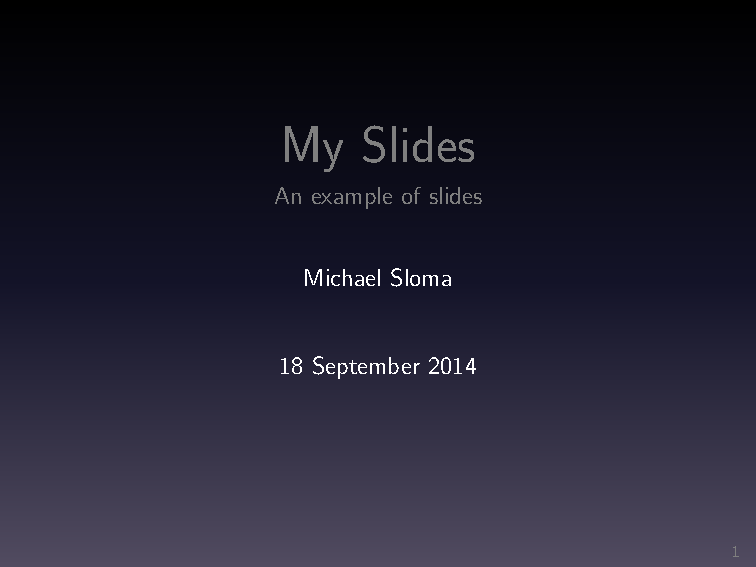
\includegraphics[height=215pt]{ex.pdf}
\end{figure}
\end{frame}

\begin{frame}{Two pictures}
\begin{figure}
        \centering
        \begin{subfigure}[a]{0.5\textwidth}
                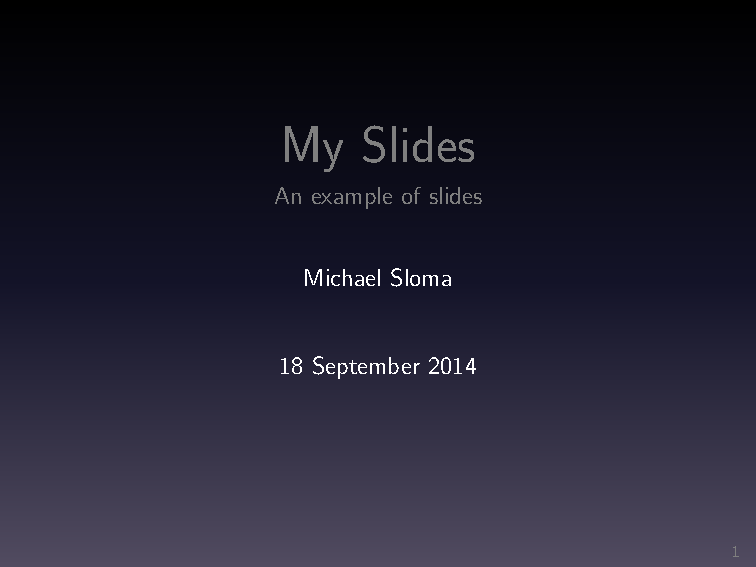
\includegraphics[height=100pt]{ex.pdf}
                \caption*{example2.tex}
        \end{subfigure}%
        \begin{subfigure}[a]{0.5\textwidth}
                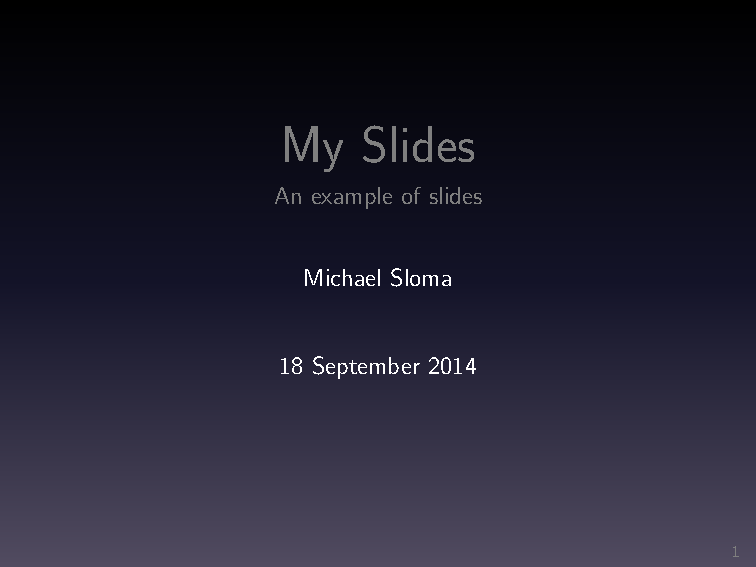
\includegraphics[height=100pt]{ex.pdf}
                \caption*{example2.pdf}
        \end{subfigure}
\end{figure}
\end{frame}

\end{document}
